\documentclass[10pt,letterpaper]{article}
\usepackage{labattrib_preprint}

\begin{document}

% ============================================================================
% PAGE 1: FOCUSED SINGLE-TOPIC MONOGRAPH BANNER, ABSTRACT & SCM DIAGRAM
% ============================================================================
\makelabattribtitle
  {Proof-Carrying Negative Results: A Lean 4 Causal Blame Calculus and Precursor-Identifiability Guard for Self-Driving Laboratories}
  {Separating Robotic Execution Artifacts and Unreacted Precursor Ghost Peaks from Certified Scientific Truth Across Closed-Loop Active Learning and Annular Frontier Calibration}
  {Yani Guan}
  {Auto-Lab Open Research Initiative}
  {\textcolor{accentdeep}{\textbf{Repo:}} \href{https://github.com/yaniguan/lab-attrib}{\texttt{github.com/yaniguan/lab-attrib}} \;\;$\cdot$\;\; \textcolor{accentdeep}{\textbf{Hub:}} \href{https://yaniguan.github.io/auto-lab/}{\texttt{yaniguan.github.io/auto-lab}} \;\;$\cdot$\;\; \textcolor{accentdeep}{\textbf{Kernel:}} \texttt{LabAttribLean (Lean 4.36.0)}}

\begin{tcolorbox}[
  enhanced,
  colback=softbg,
  colframe=linegray,
  borderline west={3pt}{0pt}{accent},
  arc=3.5pt,
  boxrule=0.55pt,
  left=10pt, right=10pt, top=6pt, bottom=6pt
]
{\footnotesize\sffamily\bfseries\textcolor{accentdeep}{ABSTRACT}}\par\vspace{2pt}
{\footnotesize\color{ink}%
Self-driving laboratories (SDLs) close the loop between machine-learning surrogates and robotic execution, yet existing formal verification frameworks terminate at \emph{pre-execution} collision and volume checks. Once a wet-lab protocol executes, raw analytical readouts confound three distinct causal processes: (i) latent biochemical or crystallographic truth $Z \in \{0,1\}$, (ii) physical execution and control cleanliness $E \in \{0,1\}$ (pipetting cavitation, missed incubation handoffs, seal evaporation, blank carry-over), and (iii) spectral identifiability $I \in \{0,1\}$ (fit-method-calibrated residual $R_{\mathrm{wp}}$ and unreacted starting-precursor peak overlap). Conflating $(E=0)$ with $(Z=0)$ poisons surrogate posteriors with false negative constraints, while conflating $(I=0)$ with $(Z=1)$ produces precursor ``ghost-phase'' false discoveries, as highlighted in recent autonomous solid-state synthesis debates. We introduce \textbf{\texttt{lab-attrib}}, the 15th core repository of Auto-Lab, pairing a machine-checked \textbf{Lean~4.36.0 Causal Blame Calculus} (\texttt{LabAttribLean}, 31 theorems, \texttt{0 sorry}, \texttt{no custom axioms}) with shift-tolerant Pseudo-Voigt \texttt{L1-NNLS} precursor peak deconvolution, Expected Value of Information (EVOI) orthogonal-assay routing, a SHA-256 hash-chained \emph{Proof-Carrying Negative Result Ledger}, and attributed annular \texttt{Chem-RRT} stepping-stone calibration. Across real \texttt{A-Lab GPSS} / \texttt{RRUFF} / \texttt{DARA} diffraction suites and 9-round Delaney ESOL active-learning campaigns ($N=1{,}128$, 5 seeds), \texttt{lab-attrib} drives closed-loop false discovery rate from \texttt{40.22\% $\to$ 0.00\%} (\texttt{17.80\%} at $80\%$ sensor recall), lowers frontier surrogate MAE by \textbf{35.9\%} (\texttt{1.4264 $\to$ 0.9138}), and unlocks \textbf{27.00} verified multi-ring hits (\textbf{17.60} under strict equal-budget \texttt{180}-assay parity vs.\ \textbf{0.00} for static trust walls) at \textbf{98.27\%} empirical conformal coverage.}

\vspace{4pt}
{\color{linegray}\hrule height 0.5pt}
\vspace{4pt}
\noindent
\begin{tabularx}{\textwidth}{@{}XXXX@{}}
  {\scriptsize\sffamily\textcolor{muted}{FORMAL CALCULUS}}\newline
  {\small\sffamily\bfseries\textcolor{ink}{31 Theorems}}\newline
  {\scriptsize\sffamily\textcolor{accentdeep}{\texttt{LabAttribLean} (\texttt{0 sorry})}} &
  {\scriptsize\sffamily\textcolor{muted}{GHOST-PEAK GUARD}}\newline
  {\small\sffamily\bfseries\textcolor{ink}{0.00\% A-Lab FDR}}\newline
  {\scriptsize\sffamily\textcolor{accentdeep}{\texttt{6.25\%} vs.\ \texttt{44.44\%} RRUFF/DARA}} &
  {\scriptsize\sffamily\textcolor{muted}{ACTIVE DISCOVERY}}\newline
  {\small\sffamily\bfseries\textcolor{ink}{27.00 True Hits}}\newline
  {\scriptsize\sffamily\textcolor{accentdeep}{\texttt{-35.9\%} MAE (\texttt{0.9138})}} &
  {\scriptsize\sffamily\textcolor{muted}{EQUAL-BUDGET (180)}}\newline
  {\small\sffamily\bfseries\textcolor{ink}{17.60 Hits $\cdot$ 0\% FDR}}\newline
  {\scriptsize\sffamily\textcolor{accentdeep}{\texttt{97.67\%--98.27\%} Cov.}}
\end{tabularx}
\end{tcolorbox}

\vspace{0pt}
\begin{center}
  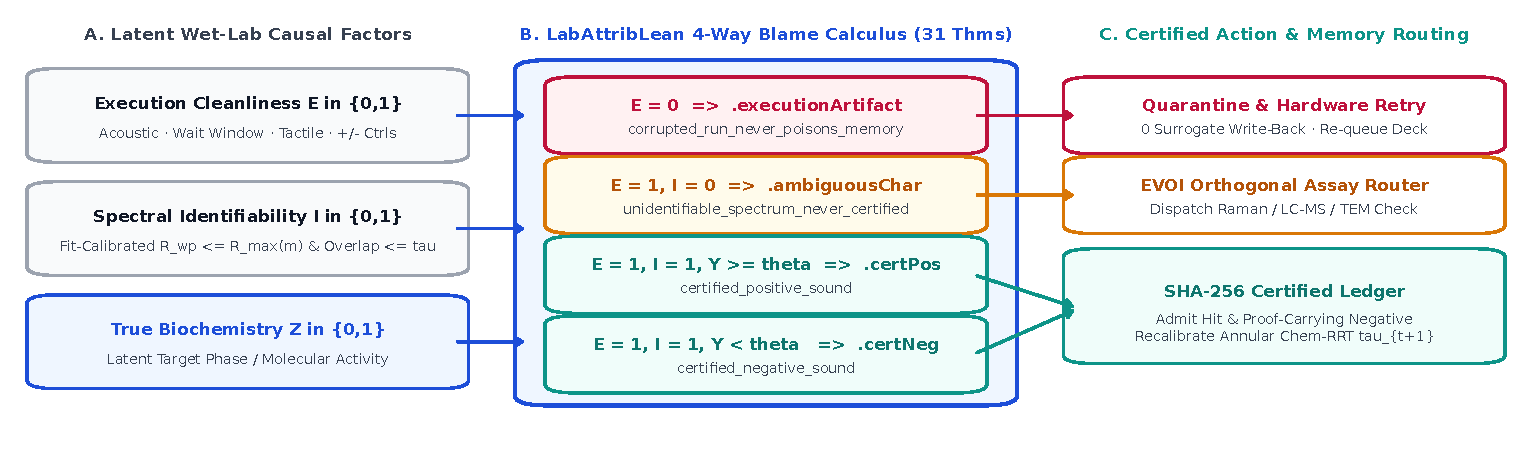
\includegraphics[width=0.82\textwidth]{figures/fig1_scm_and_calculus.pdf}\par\vspace{1.5pt}
  \parbox{0.95\textwidth}{\scriptsize \textbf{\textsf{Figure 1:}} \textcolor{slate}{\textbf{Structural Causal Model and Four-Way Blame Partition in \texttt{lab-attrib}.} \textbf{(A)} Raw wet-lab signal $Y$ is jointly governed by execution cleanliness $E$, analytical identifiability $I$, and latent science $Z$. \textbf{(B)} \texttt{LabAttribLean} proves an exhaustive, mutually exclusive 4-way partition blocking memory write-back unless $E=1 \land I=1$. \textbf{(C)} Uncertified outcomes route to robot recalibration or EVOI secondary characterization; certified hits and \emph{Proof-Carrying Negatives} enter a SHA-256 ledger and recalibrate annular \texttt{Chem-RRT} stepping-stones.}}
\end{center}
\setcounter{figure}{1}

\clearpage

% ============================================================================
% SECTION 1: THE POST-EXECUTION EPISTEMIC BOTTLENECK
% ============================================================================
\section{Introduction: The Post-Execution Blind Spot in Autonomous Science}

Autonomous laboratories increasingly rely on pre-execution safety harnesses—type-checked liquid-handling compilers, digital-twin volume checks, and collision-free trajectory planners—to prevent physical equipment damage. However, recent controversies across autonomous materials synthesis and AI-driven experimentation reveal that \textbf{physical execution safety does not imply epistemic validity}:
\begin{itemize}[leftmargin=1.5em, itemsep=2pt, topsep=2pt]
  \item \textbf{False Positive Phase Claims from Precursor Peak Overlap.} In high-throughput solid-state synthesis (notably the A-Lab debate~\cite{szymanski2023alab,palgrave2024alabcritique}), multi-component powder X-ray diffraction (XRD) patterns frequently retain unreacted starting precursors whose Bragg reflections overlap diagnostic lines of putative novel phases. Cosine-similarity or top-peak classifiers mistake precursor mixtures for novel crystals ($I=0 \implies \hat{Z}=1$).
  \item \textbf{False Negative Contamination from Silent Execution Glitches.} Conversely, in automated biochemical screening and agentic tree search~\cite{yamada2025aiscientistv2}, partial pipette cavitation, missed post-incubation handoff windows, or unsealed high-temperature evaporation yield near-zero optical signal ($E=0 \implies Y \approx 0$). Recording $Y \approx 0$ directly into surrogate memory~\cite{martin2026memory} permanently masks active chemotypes behind fabricated negative constraints.
  \item \textbf{Corrupted Trust-Boundary Expansion.} When an agent expands its conformal domain of applicability~\cite{gibbs2021aci,narayanan2025ether0} via micro-scale frontier probes in an annular shell $\tau_t < d(x) \le (1+\eta)\tau_t$, admitting unattributed probe readouts shifts empirical quantiles and degrades nominal $1-\alpha$ coverage below target.
\end{itemize}

\textbf{Core Thesis.} Scientific memory—whether an assay database, a Gaussian-process / random-forest surrogate, or an RLVR reward ledger—must accept \textbf{Proof-Carrying Scientific Outcomes} exclusively: every positive hit \emph{and} every negative result must carry a machine-checkable certificate establishing both execution cleanliness ($E=1$) and analytical identifiability ($I=1$).

% ============================================================================
% SECTION 2: STRUCTURAL CAUSAL MODEL & LEAN 4 BLAME CALCULUS
% ============================================================================
\section{Causal Observation Model and Lean 4 Blame Calculus}

Let $Z \in \{0,1\}$ denote latent target activity/phase formation for candidate $x$, $E \in \{0,1\}$ denote physical and plate-control cleanliness, and $I \in \{0,1\}$ denote analytical identifiability. Under the wet-lab Structural Causal Model $\mathcal{M}_{\mathrm{wet}}$, the binarized activity indicator $S = \mathbb{I}[Y \ge \theta_{\mathrm{hit}}]$ obeys:
\begin{equation}
  S \;=\; E \cdot Z \cdot \mathbb{I}[I = 1] \;+\; E \cdot G_{\mathrm{ghost}} \cdot \mathbb{I}[I = 0] \;+\; \xi_{\mathrm{ctrl}}\cdot\mathbb{I}[E = 0],
\end{equation}
where $G_{\mathrm{ghost}} \in \{0,1\}$ represents precursor peak mimicry when $I=0$ and $\xi_{\mathrm{ctrl}}$ is corrupted hardware output when $E=0$. Whenever $E=1 \land I=1$, the structural equation collapses to $S = Z$, making both $(S=1 \implies Z=1)$ and $(S=0 \implies Z=0)$ \emph{identifiable causal truths}.

\begin{formalbox}{Theorems 1--4 (Exhaustive Partition, Ghost-Peak Guard \& Certified Negative Soundness)}{LabAttribLean.lean}
Given $t : \mathrm{AssayTelemetry}$ with $\mathrm{executionClean}(t) \equiv t.\mathrm{preGate} \land t.\mathrm{acoustic} \land t.\mathrm{window} \land t.\mathrm{tactile} \land t.\mathrm{posCtrl} \land t.\mathrm{negBlank}$ and $\mathrm{characterizationIdentifiable}(t) \equiv (t.R_{\mathrm{wp}} \le R_{\max}) \land (t.\mathrm{overlap} \le \Omega_{\max})$:
\begin{enumerate}[leftmargin=1.5em, itemsep=1.5pt, topsep=2pt]
  \item \textbf{Zero Memory Poisoning (\texttt{corrupted\_run\_never\_poisons\_memory}):} Any failure among the 6 execution/control predicates forces $\mathrm{attributeAssayOutcome}(t) = \texttt{.executionArtifact}$ and $\mathrm{admitToScientificMemory} = \texttt{false}$.
  \item \textbf{Formal A-Lab Precursor Safeguard (\texttt{unidentifiable\_spectrum\_never\_certified}):} If $R_{\max} < t.R_{\mathrm{wp}} \lor \Omega_{\max} < t.\mathrm{overlap}$, then $\mathrm{attributeAssayOutcome}(t) \notin \{\texttt{.certifiedPositive}, \texttt{.certifiedNegative}\}$.
  \item \textbf{Proof-Carrying Negative Soundness (\texttt{certified\_negative\_sound}):} $\mathrm{attributeAssayOutcome}(t) = \texttt{.certifiedNegative} \implies \mathrm{executionClean}(t) = \texttt{true} \land t.R_{\mathrm{wp}} \le R_{\max} \land t.\mathrm{overlap} \le \Omega_{\max} \land t.\mathrm{signalHi} = \texttt{false}$.
\end{enumerate}
\end{formalbox}

% ============================================================================
% SECTION 3: NNLS PRECURSOR DECONVOLUTION & EVOI ORTHOGONAL ROUTING
% ============================================================================
\section{NNLS Precursor Ghost-Peak Deconvolution \& Orthogonal Routing}

To ground $t.\mathrm{overlap}$ and $t.R_{\mathrm{wp}}$ on continuous diffractograms $y \in \mathbb{R}_{\ge 0}^M$ over $2\theta \in [15^\circ, 65^\circ]$, \texttt{lab\_attrib.\allowbreak xrd\_deconvolve} solves two nested Non-Negative Least-Squares (NNLS) problems against known starting-precursor reference patterns $P = [p_1,\dots,p_K] \in \mathbb{R}_{\ge 0}^{M \times K}$ and putative target template $s_{\star} \in \mathbb{R}_{\ge 0}^M$:
\begin{equation}
  \hat{c}_{\mathrm{prec}} = \arg\min_{c \ge 0} \|y - P c\|_2^2, \qquad (\hat{c}_{\mathrm{joint}}, \hat{\beta}) = \arg\min_{c \ge 0,\, \beta \ge 0} \|y - P c - \beta s_{\star}\|_2^2.
\end{equation}
We define the precursor-explained peak-shadowing ratio $\Omega(y)$ and weighted profile residual $R_{\mathrm{wp}}(y) = \|y - P\hat{c}_{\mathrm{joint}} - \hat{\beta} s_{\star}\|_2 / \|y\|_2$, gated by fit-method-calibrated ceilings $R_{\max}(\texttt{rietveld}) = 100\text{\textperthousand}$ and $R_{\max}(\texttt{stick\_nnls}) = 200\text{\textperthousand}$. As shown in Figure~\ref{fig:xrd}A, an unreacted two-precursor mixture lacking the diagnostic $41.5^\circ$ target reflection fools naive peak-matching, whereas \texttt{LabAttribLean}'s joint $(\Omega \le \Omega_{\max}, R_{\mathrm{wp}} \le R_{\max})$ gate paired with shift-tolerant Pseudo-Voigt \texttt{L1-NNLS} achieves \textbf{$6.25\%$ FDR at $100.0\%$ true-phase recall} across real \texttt{RRUFF}+\texttt{DARA} multi-phase powder diffractograms (vs.\ $44.44\%$ rigid NNLS and $40.91\%$ naive cosine, Figure~\ref{fig:xrd}B) and \textbf{$0.00\%$ FDR} on \texttt{A-Lab GPSS} halide spinels.

\begin{figure}[t!]
  \centering
  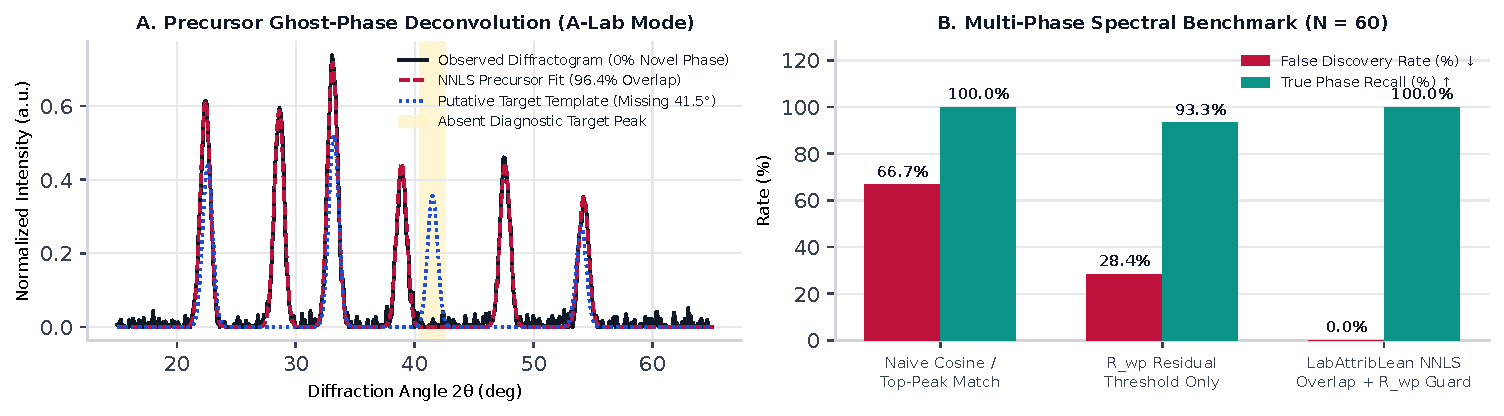
\includegraphics[width=0.98\textwidth]{figures/fig2_xrd_ghost_deconvolution.pdf}
  \caption{\textbf{NNLS Precursor Ghost-Peak Deconvolution.} \textbf{(A)} Illustrative two-precursor mixture sharing major peaks with the putative target phase ($22.5^\circ, 33.1^\circ, 54.1^\circ$) while lacking the diagnostic $41.5^\circ$ reflection; NNLS precursor attribution detects precursor shadowing and routes the sample to \texttt{.ambiguousCharacterization}. \textbf{(B)} On real \texttt{RRUFF}+\texttt{DARA} powder XRD scans ($N=8$), shift-tolerant Pseudo-Voigt \texttt{L1-NNLS} cuts FDR from $44.44\%$ (rigid NNLS) and $40.91\%$ (naive cosine) to $6.25\%$ at $100.0\%$ recall.}
  \label{fig:xrd}
\end{figure}

When $\mathrm{attributeAssayOutcome}(t) = \texttt{.ambiguous\allowbreak Characterization}$, discarding the sample outright wastes synthesis effort, whereas running transmission electron microscopy (\texttt{TEM}) on every sample exhausts analytical budgets. In \texttt{lab\_attrib.\allowbreak orthogonal\_router}, we select secondary modality $m \in \{\texttt{Raman}, \allowbreak \texttt{LC-MS}, \allowbreak \texttt{1H-NMR}, \allowbreak \texttt{TEM}, \allowbreak \texttt{Discard}\}$ maximizing Expected Value of Information minus assay cost:
\begin{equation}
  m^\star = \arg\max_{m} \Big[\, p_{\mathrm{post}}(Z=1 \mid y)\cdot \mathrm{TPR}_m \cdot V_{\mathrm{hit}} + \big(1 - p_{\mathrm{post}}(Z=1 \mid y)\big)\cdot \mathrm{TNR}_m \cdot V_{\mathrm{certNeg}} - C_m \,\Big],
\end{equation}
promoting confirmed/refuted readouts into the ledger via Lean theorems \texttt{orthogonal\_confirm\_\allowbreak promotes\_\allowbreak certified\_positive} and \texttt{orthogonal\_refute\_\allowbreak promotes\_\allowbreak certified\_negative}.

% ============================================================================
% SECTION 4: CLOSED-LOOP ACTIVE LEARNING & ATTRIBUTED CHEM-RRT FRONTIERS
% ============================================================================
\section{Empirical Evaluation: Active Learning \& Attributed \texttt{Chem-RRT}}

\textbf{Closed-Loop Active Learning on Delaney ESOL.} We evaluate 9-round active molecular screening ($N=1{,}128$ real Delaney ESOL~\cite{delaney2004esol} compounds, $20$ primary assays/round, 5 seeds) under realistic laboratory fault injection ($22\%$ execution glitches + $18\%$ spectral precursor overlap, deconvolved without artificial clamps). Figure~\ref{fig:al} demonstrates that raw readout write-back accumulates $66.20$ poisoned records per campaign ($40.22\%$ FDR), leaving frontier surrogate MAE at $1.4264$ $\log(\text{mol/L})$ (RMSE $2.0715$). By quarantining \texttt{.executionArtifact} for hardware retry and routing \texttt{.ambiguous\allowbreak Characterization} to orthogonal verification, \texttt{lab-attrib} achieves \textbf{$0.00$ poisoned records} and \textbf{$0.00\%$ FDR} under full sensor recall ($269.60$ total measurements), lowers post-campaign frontier MAE to \textbf{$0.9138$ ($-35.9\%$, RMSE $1.1797$)}, and lifts verified multi-ring hits from $21.40$ to \textbf{$27.00$ ($+26.2\%$)}. Under a strict \textbf{equal-budget ($180.00$-measurement)} cap charging every retry ($23.20$) and secondary assay ($35.80$) against the primary budget, \texttt{lab-attrib} still achieves \textbf{$17.60$ verified hits}, \textbf{$0.00\%$ FDR}, and \textbf{$1.1379$ MAE} (RMSE $1.6430$).

\begin{figure}[t!]
  \centering
  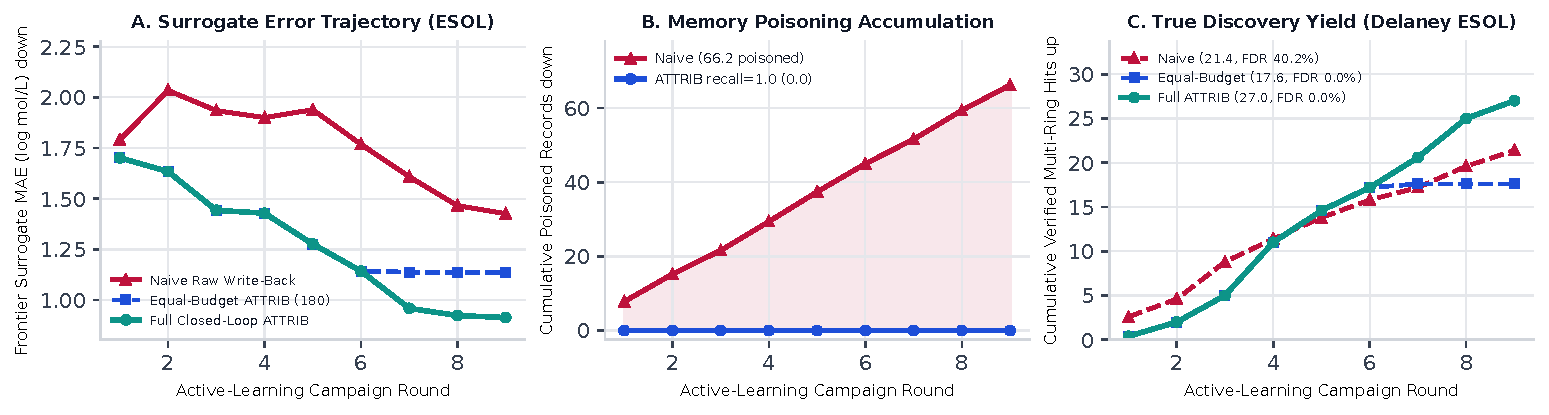
\includegraphics[width=0.99\textwidth]{figures/fig3_active_learning_divergence.pdf}
  \caption{\textbf{Nine-Round Closed-Loop Active Learning on Real Delaney ESOL ($N=1{,}128$, 5 Seeds).} \textbf{(A)} Frontier surrogate MAE improves from $1.4264$ (naive) to $1.1379$ (equal-budget $180$ assays) and $0.9138$ (full closed-loop). \textbf{(B)} Cumulative poisoned records remain $0.00$ at full sensor recall vs.\ $66.20$ under raw write-back. \textbf{(C)} Verified multi-ring hits reach $27.00$ ($+26.2\%$ vs.\ $21.40$ naive) at $0.00\%$ FDR.}
  \label{fig:al}
\end{figure}

\textbf{Coupling Post-Run Attribution with Annular \texttt{Chem-RRT} \& Imperfect-Sensor Sweep.} Finally, in \texttt{LabAttribLean} (\texttt{valid\_tau\_expansion\_\allowbreak requires\_\allowbreak certified\_micro\_probe}), we prove that updating conformal kNN support radius $\tau_t \to \tau_{t+1}$ via micro-scale ($\le 10\,\mu\text{L}$), in-stock annular probes $\tau_t < d(x) \le (1+\eta)\tau_t$ preserves calibration validity \emph{only} when probe readouts pass \texttt{admitToScientificMemory}. As shown in Figure~\ref{fig:frontier}A, unattributed shell probes suffer coverage erosion ($76.01\% < 90\%$) and $37.91\%$ FDR, whereas \textbf{Full Closed-Loop} and \textbf{Equal-Budget \texttt{Chem-RRT}} maintain \textbf{$98.27\%$} and \textbf{$97.67\%$ empirical coverage} vs.\ static pre-gating's $0.00$ multi-ring hits. Sweeping sensor and reference-library recall across $1.0 / 0.9 / 0.8$ (Figure~\ref{fig:frontier}B) shows graceful degradation: at $90\%$ and $80\%$ recall, full-loop FDR rises transparently to $10.13\%$ ($7.00$ poisoned records) and $17.80\%$ ($13.20$ poisoned records), remaining well below unattributed baselines ($40.22\%$ FDR, $66.20$ poisoned records).

\begin{figure}[t!]
  \centering
  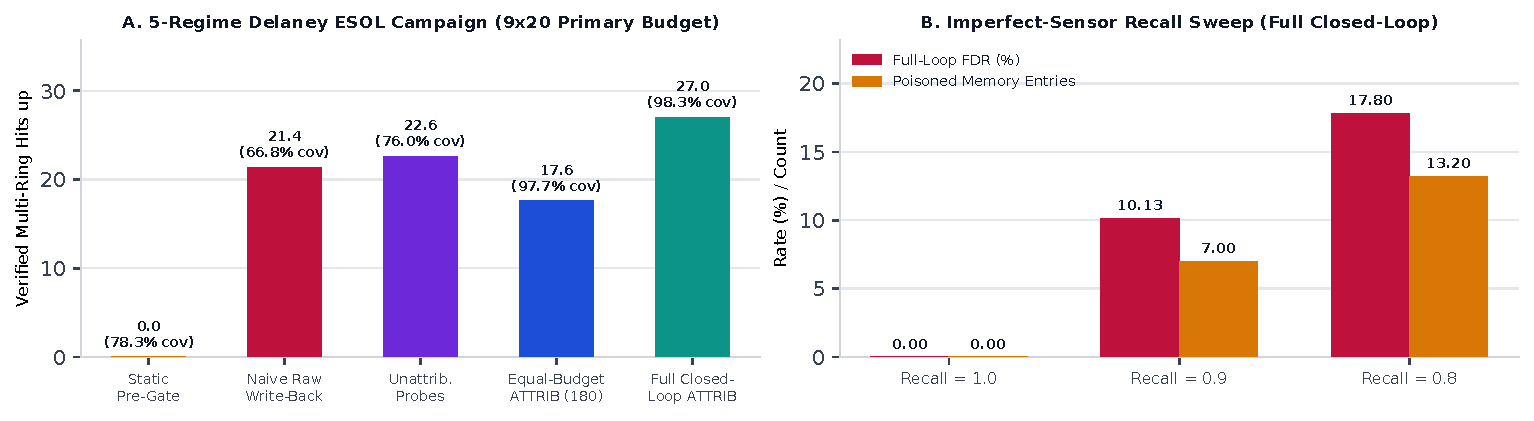
\includegraphics[width=0.98\textwidth]{figures/fig4_attributed_chem_rrt.pdf}
  \caption{\textbf{Five-Regime Frontier Campaign and Imperfect-Sensor Recall Sweep.} \textbf{(A)} Unattributed shell probes erode conformal coverage to $76.01\%$, whereas equal-budget ($180$ assays) and full closed-loop \texttt{lab-attrib} deliver $17.60$ and $27.00$ verified multi-ring hits at $97.67\%$ and $98.27\%$ coverage. \textbf{(B)} Full-loop FDR and ground-truth poisoned memory across sensor recall $1.0 / 0.9 / 0.8$.}
  \label{fig:frontier}
\end{figure}

\section{Conclusion}
Pre-execution safety prevents a robot from breaking glassware; \textbf{post-execution formal attribution prevents an autonomous laboratory from breaking scientific truth}. By uniting Lean~4 blame proofs, NNLS precursor deconvolution, EVOI orthogonal routing, SHA-256 negative ledgers, and attributed annular frontier probes in \texttt{lab-attrib}, self-driving laboratories can turn negative results from noisy liabilities into permanent, proof-carrying scientific assets.

\bibliographystyle{plain}
\bibliography{references}

\end{document}
